\documentclass[
	% -- opções da classe memoir --
	12pt,				% tamanho da fonte
	%openright,			% capítulos começam em pág ímpar (insere página vazia caso preciso)
	oneside,			% p/ impressão frente e verso:
	%					%oneside -> Normal. 
	%					%twoside -> insere página antes e depois de cada capítulo
	a4paper,			% tamanho do papel. 
	% -- opções da classe abntex2 --
	%chapter=TITLE,		% títulos de capítulos convertidos em letras maiúsculas
	%section=TITLE,		% títulos de seções convertidos em letras maiúsculas
	%subsection=TITLE,	% títulos de subseções convertidos em letras maiúsculas
	%subsubsection=TITLE,% títulos de subsubseções convertidos em letras maiúsculas
	% -- opções do pacote babel --
	english,			% idioma adicional para hifenização
	french,				% idioma adicional para hifenização
	spanish,			% idioma adicional para hifenização
	brazil				% o último idioma é o principal do documento
	]{abntex2}
% ---
% Pacotes básicos 
% ---
\usepackage{lmodern}			% Usa a fonte Latin Modern			
\usepackage[T1]{fontenc}		% Selecao de codigos de fonte.
\usepackage[utf8]{inputenc}		% Codificacao do documento (conversão automática dos acentos)
\usepackage{indentfirst}		% Indenta o primeiro parágrafo de cada seção.
\usepackage{color}				% Controle das cores
\usepackage{graphicx}			% Inclusão de gráficos
\usepackage{microtype} 			% para melhorias de justificação
\usepackage{steinmetz}          % Notação fasorial
\usepackage{paracol}            % Criar colunas

% ---
% Atribuições Matemáticas 
% ---
\usepackage{amsmath, amsfonts, amssymb} % pacotes para caracteres extras
\DeclareMathOperator{\sen}{sen}
\DeclareMathOperator{\arcsen}{arcsen}
\DeclareMathOperator{\tg}{tg}
\DeclareMathOperator{\cossec}{cossec}
\newcommand{\limite}{\displaystyle\lim}
\newcommand{\integral}{\displaystyle\int}
		
% ---
% Pacotes de citações
% ---
\usepackage[brazilian,hyperpageref]{backref}	 % Paginas com as citações na bibl
\usepackage[alf]{abntex2cite}	% Citações padrão ABNT

% --- 
% CONFIGURAÇÕES DE PACOTES
% --- 

% ---
% Configurações do pacote backref
% Usado sem a opção hyperpageref de backref
\renewcommand{\backrefpagesname}{Citado na(s) página(s):~}
% Texto padrão antes do número das páginas
\renewcommand{\backref}{}
% Define os textos da citação
\renewcommand*{\backrefalt}[4]{
	\ifcase #1 %
		Nenhuma citação no texto.%
	\or
		Citado na página #2.%
	\else
		Citado #1 vezes nas páginas #2.%
	\fi}%
% ---

% ---
% Informações de dados para CAPA e FOLHA DE ROSTO
% ---
\titulo{TRABALHO 3: \\ \textbf{Análise do regime permanente senoidal}}
\autor{Antonio Gabriel Sousa Borralho \\ Antonio José Portela de Jesus Santos \\ Arthur Monteiro Costa Silva \\ Bruno Leal da Silva \\ Lucas Costa Soares}
\local{São Luís, MA - Brasil}
\data{\today}
%\orientador{Prof. Professor}
\tipotrabalho{Relatório Experimental}
% O preambulo deve conter o tipo do trabalho, o objetivo, 
% o nome da instituição e a área de concentração 
\preambulo{Trabalho referente à resolução das questões da terceira lista de exercícios, para obtenção parcial da terceira nota da disciplina Circuitos Elétricos no período de 2018.1.\newline \newline Prof. Luciano Buonocore.}
% ---


% ---
% Configurações de aparência do PDF final

% alterando o aspecto da cor azul
\definecolor{blue}{RGB}{41,5,195}

% informações do PDF
\makeatletter

\hypersetup{
     	%pagebackref=true,
		pdftitle={\@title}, 
		pdfauthor={\@author},
    	%pdfsubject={\imprimirpreambulo},
	    pdfcreator={LaTeX with abnTeX2},
		pdfkeywords={abnt}{latex}{abntex}{abntex2}{trabalho acadêmico}, 
		colorlinks=true,       		% false: boxed links; true: colored links
    	linkcolor=blue,          	% color of internal links
    	citecolor=blue,        		% color of links to bibliography
    	filecolor=magenta,          % color of file links
		urlcolor=blue,
		bookmarksdepth=4
}

\makeatother
% --- 

% --- 
% Espaçamentos entre linhas e parágrafos 
% --- 

% O tamanho do parágrafo é dado por:
\setlength{\parindent}{1.3cm}

% Controle do espaçamento entre um parágrafo e outro:
\setlength{\parskip}{0.2cm}  % tente também \onelineskip

% ---
% compila o indice
% ---
\makeindex
% ---

% ----
% Início do documento
% ----
\begin{document}

% Seleciona o idioma do documento (conforme pacotes do babel)
%\selectlanguage{english}
\selectlanguage{brazil}

% Retira espaço extra obsoleto entre as frases.
\frenchspacing 

% ----------------------------------------------------------
% ELEMENTOS PRÉ-TEXTUAIS
% ----------------------------------------------------------
\pretextual
% ---
% --------------------- CAPA -------------------------------
% ---
\begin{center}			
	\begin{figure}[htb]
		\centering
		
\includegraphics[scale=0.15]{ufmalogo.jpg}
	\end{figure}
				
			\textbf{UNIVERSIDADE FEDERAL DO MARANHÃO \\
					CENTRO DE CIÊNCIAS EXATAS E TECNOLOGIAS \\
					DEPARTAMENTO DE ENGENHARIA ELÉTRICA \\
				    CIRCUITOS ELÉTRICOS\\\vspace{4cm}}
					
					\textbf{\large{TRABALHO 3:}\\
					\large{Análise do regime permanente senoidal}}
					\vspace{3.5cm}
					\begin{flushright}
						\textnormal{Antonio Gabriel Sousa Borralho \\ Antonio José Portela de Jesus Santos \\ Arthur Monteiro Costa Silva \\ Bruno Leal da Silva \\ Lucas Costa Soares}
					\end{flushright}
					\vspace{3.5cm}
					\textbf{São Luís, MA - Brasil\\ \today}
\end{center}
% ---
% --------------------- FOLHA DE ROSTO -------------------------------
% ---
\renewcommand{\folhaderostocontent}{  % Cria sua própria folha de rosto 
    \begin{center}
        % ____Autores_________________________________________
        {\ABNTEXchapterfont\imprimirautor}
        \vspace*{\fill}\vspace*{\fill}
        % ____Título_________________________________________
        \begin{center}
            \ABNTEXchapterfont\bfseries\Large\imprimirtitulo
        \end{center}
        \vspace*{\fill}
        % ____Pré-Ambulo_________________________________________
        \abntex{}{%
            \hspace{.45\textwidth}
            \begin{minipage}{.5\textwidth}
                \SingleSpacing
                \imprimirpreambulo
            \end{minipage}%
            \vspace*{\fill}
        }%
        % ____Instituição_______________________________________
        %{\abntex{\imprimirinstituicao}{\imprimirinstituicao
        %\vspace*{\fill}}}
        % ____Orientador_________________________________________
        %{\large\imprimirorientadorRotulo~\imprimirorientador\par}
        % ____Co-Orientador___________________________________
        %\abntex{\imprimircoorientador}{%
        %    {\large\imprimircoorientadorRotulo~\imprimircoorientador}%
        %}%
        % ____Local/Data______________________________________
        {\large\imprimirlocal}
        \par
        {\large\imprimirdata}
        %\vspace*{1cm}
    \end{center}
}
\makeatother
% ---
% Folha de rosto
% (o * indica que haverá a ficha bibliográfica)
% ---
\imprimirfolhaderosto

% ---
% --------------------- SUMÁRIO -------------------------------
% ---
\pdfbookmark[0]{\contentsname}{toc}
\tableofcontents*
\cleardoublepage
% ---

% ----------------------------------------------------------
% ELEMENTOS TEXTUAIS
% ----------------------------------------------------------
\textual
% ----------------------------------------------------------
% Introdução (exemplo de capítulo sem numeração, mas presente no Sumário)
% ----------------------------------------------------------
\chapter{Conceitos Básicos}
% ----------------------------------------------------------

Circuitos com \textbf{resistores, capacitores e indutores} denominados $RLC$, que apesar de sua simplicidade, têm inúmeras aplicações em eletrônica, comunicação e sistemas de controle \cite{sadiku}. Assim como outros, esses componentes são mais fáceis de descrever em termos de variáveis de circuito do que de variáveis eletromagnéticas. No entanto, antes de nos concentrarmos na descrições desses elementos do ponto de vista de circuitos, é recomendável realizarmos uma breve revisão dos conceitos de campo a eles subjacentes. 

Um indutor é um componente elétrico que se opõe a qualquer mudança na corrente elétrica. É composto por uma bobina de fio enrolado em torno de um núcleo de suporte cujo material pode ser magnético ou não magnético. O comportamento dos indutores é baseado em fenômenos associado a campos magnéticos. Um  campo magnético que varia com o tempo induz uma tensão em qualquer condutor imerso ao campo. O parâmetro \textbf{indutância} relaciona a tensão induzida com a corrente. Um capacitor é um componente elétrico que consiste em dois condutores separados por um isolante ou material dielétrico. O capacitor é o único dispositivo, além da bateria, que pode armazenar carga elétrica. O comportamento dos capacitores é baseado em fenômenos associados a campos elétricos. Um campo elétrico que varia com o tempo produz uma corrente de deslocamento no espaço ocupado pelo campo. O parâmetro \textbf{capacitância} relaciona a corrente de deslocamento à tensão, onde a corrente de deslocamento é igual à corrente de condução nos terminais do capacitor.

Neste trabalho temos interesse em resolver problemas em que a fonte de tensão ou corrente varie senoidalmente. Fontes senoidais e seus efeitos sobre o comportamento do circuito são uma importante área de estudo por várias razões. Em primeiro lugar, geração, transmissão, distribuição e consumo de energia elétrica ocorrem sob condições de \textbf{regime permanente} essencialmente senoidais. A segunda razão é que o entendimento do regime senoidal torna possível a previsão do comportamento de circuitos com fontes não senoidais. A terceira é que o comportamento de regime permanente senoidal costuma simplificar o projeto de sistemas elétricos. Assim, um projetista que formula claramente suas especificações em termos de uma resposta de regime permanente senoidal desejável e projetar o circuito ou sistema para satisfazer essas características. Se o dispositivo atende às especificações, o projetista sabe que o circuito responderá satisfatoriamente a entradas não senoidais.
\cite{nilssonriedel}
%=====================================================================================================================================================
%====== QUESTÕES ===============================================================================================================================================
\chapter{Questões}

% ----------------------------------------------------------
% QUESTÃO 3.2
% ----------------------------------------------------------

\section*{Questão 3.2}
\addcontentsline{toc}{section}{Questão 3.2}
No circuito 3.2, as fontes operam em $\omega$=1 rad/s. Se \textbf{I$_C$} = 2$\;\phase{28^{\circ}}\;A$ e \textbf{I$_L$} = 3$\;\phase{53^{\circ}}\;A$. Determine: a)\textbf{I$_S$} ; b)\textbf{V$_S$} ; c) $i_R__1$(t)
\begin{figure}[htb]
	\centering
	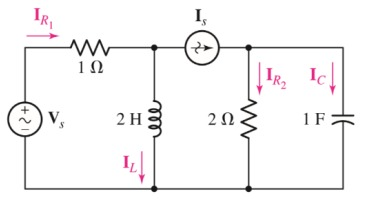
\includegraphics[scale=0.65]{3-02.jpeg}
	\caption{Circuito 3.2}
\end{figure}
\begin{figure}[htb]
	\centering
	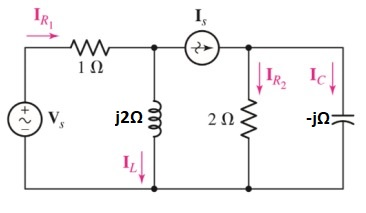
\includegraphics[scale=1]{3-02-2.jpeg}
	\caption{Circuito no domínio da frequência}
\end{figure}
%--3.2 - Letra A -------------------------------------------------------------------------------------
\newline
$a)$ Para saber \textbf{I$_S$}, devemos saber a tensão no capacitor \textbf{V$_C$} para assim calcular a corrente \textbf{I$_R__2$} e por LCK calcular \textbf{I$_S$} :

\newline

Primeiramente, calculando a impedância capacitiva \textbf{Z$_C$}, temos:

\begin{equation}
    \centering
    \textbf{Z$_C$}=-\textbf{j}\cdot(\frac{1}{\omega\cdot C})=-\textbf{j}\cdot(\frac{1}{1\cdot 1})=-\textbf{j}\;\Omega
    \longrightarrow
    \fbox{\textbf{Z$_C$}\;=\;1\;\phase{-90^{\circ}}\;\Omega}
\end{equation}

Tendo o valor de \textbf{Z$_C$}, podemos calcular \textbf{V$_C$}:

\begin{equation}
    \centering
    \textbf{V$_C$}=\textbf{Z$_C$}\cdot\textbf{I$_C$}=1\;\phase{-90^{\circ}}\cdot 2\;\phase{28^{\circ}}
    \longrightarrow
    \fbox{\textbf{V$_C$}\;=\;2\;\phase{-62^{\circ}}\;V}
\end{equation}

Calculando a corrente \textbf{I$_R__2$}:

\begin{equation}
    \centering
    \textbf{I$_R__2$}=\frac{\textbf{V$_C$}}{\textbf{$R__2$}}=\frac{2\;\phase{-62^{\circ}}}{2\;\phase{0^{\circ}}}
    \longrightarrow
    \fbox{\textbf{I$_R__2$}=1\;\phase{-62^{\circ}}\;A}
\end{equation}

Por LCK, temos que:

\begin{equation}
    \centering
    \textbf{I$_S$}=\textbf{I$_R__2$}+\textbf{I$_C$}=1\;\phase{-62^{\circ}}+2\;\phase{28^{\circ}}
    \longrightarrow
    \fbox{\textbf{I$_S$}\;=\;2.263\;\phase{1.435^{\circ}}\;A}
\end{equation}

$b)$ Para encontrar \textbf{V$_S$}, devemos saber a corrente \textbf{I$_R__1$}, a tensão no indutor \textbf{V$_L$} e a tensão em \textbf{V$_R__1$}, e por LTK achar \textbf{V$_S$} :

Primeiramente calculando \textbf{I$_R__1$}, temos, por LCK, que:
\begin{equation}
    \centering
    \textbf{I$_R__1$}=\textbf{I$_L$}+\textbf{I$_S$}=3\;\phase{53^{\circ}}+2.236\;\phase{1.435^{\circ}}
    \longrightarrow
    \fbox{\textbf{I$_R__1$}\;=\;4.726\;\phase{31.248^{\circ}}\;A}
\end{equation}

Encontrando a tensão no indutor \textbf{V$_L$}:

Primeiramente, calculando a impedância indutiva \textbf{Z$_L$}, temos:

\begin{equation}
    \centering
    \textbf{Z$_L$}=\textbf{j}\cdot\omega\cdot L=\textbf{j}\cdot1\cdot2=\textbf{j}\cdot2\Omega
    \longrightarrow
    \fbox{\textbf{Z$_L$}\;=\;2\;\phase{90^{\circ}}\;\Omega}
\end{equation}

Tendo o valor de \textbf{Z$_L$}, podemos calcular \textbf{V$_L$}:

\begin{equation}
    \centering
    \textbf{V$_L$}=\textbf{Z$_L$}\cdot\textbf{I$_L$}=2\;\phase{90^{\circ}}\cdot 3\;\phase{53^{\circ}}
    \longrightarrow
    \fbox{\textbf{V$_L$}\;=\;6\phase{143^{\circ}}\;V}
\end{equation}

Calculando \textbf{V$_R__1$}:
\begin{equation}
    \centering
    \textbf{V$_R__1$}=\textbf{R$__1$}\cdot\textbf{I$_R__1$}=1\;\phase{0^{\circ}}\cdot4.726\;\phase{31.248^{\circ}}
    \longrightarrow
    \fbox{\textbf{V$_R__1$}\;=\;4.726\phase{31.248^{\circ}}\;V}
\end{equation}

Por LTK, temos:
\begin{equation}
    \centering
    \textbf{V$_S$}=\textbf{V$_R__1$}+\textbf{V$_L$}=4.726\;\phase{31.248^{\circ}}+6\;\phase{143^{\circ}}
    \longrightarrow
    \fbox{\textbf{V$_S$}\;=\;6.108\;\phase{97.065^{\circ}}\;V}
\end{equation}
$c)$ \textbf{I$_R__1$}\;=\;4.726\;\phase{31.248^{\circ}}\;A
\newline
Escrevendo a corrente em {$R_1$} em função do tempo, temos:
\begin{equation}
    \centering
    {i_R__1(t)}= {I_m_a_x}\cdot cos(\omega t + \theta) \;A
    \longrightarrow
    \fbox{$i_R__1$(t)= 4.726\cdot cos(1\cdot t + 31.248)\;A}
\end{equation}

\begin{flushright}
    $\Box$
\end{flushright}

\newpage

% ----------------------------------------------------------
% QUESTÃO 3.6
% ----------------------------------------------------------

\section*{Questão 3.6}
\addcontentsline{toc}{section}{Questão 3.6}
Considere o Circuito $3.6$ e determine a impedância equivalente vista a partir dos terminais abertos, se:

$(a)$ $\omega = 1\;rad/s$;

$(b)$ $\omega = 10\;rad/s$;

$(c)$ $\omega = 10\;rad/s$;

\begin{figure}[htb]
	\centering
	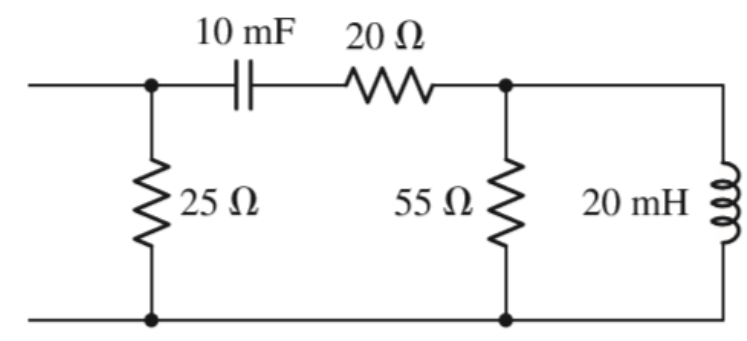
\includegraphics[scale=0.4]{3-06.PNG}
	\caption{Circuito 3.6}
\end{figure}
Inicialmente transformamos o circuito para o domínio da frequência, com base nas seguintes equações:
$$Z_L=j\omega L\;\Omega$$
$$Z_C=-j\dfrac{1}{\omega C}\;\Omega$$

%--3.6 - Letra A --------------------------------------------------------------------------
$a)$ Para $\omega = 1\;rad/s$:

Neste caso, $Z_L=j\cdot1\cdot20\cdot10^{-3} = j\cdot0,02\;\Omega$ e $Z_C=-j\frac{1}{1\cdot10\times10^{-3}}=-j100\;\Omega$.

Em seguida encontramos a impedância entre o resistor de $55\;\Omega$ em paralelo com o indutor de $20\;mH$, assim:
$$Z_L=j0,02 \Omega \;\;\; Z_C=-j100\;\Omega$$
$$Z_{eq_1} = \dfrac{55 \cdot j0,02}{55 + j0,02} = \dfrac{1,1\phase{90^\circ}}{55\phase{0,02^\circ}} = \dfrac{1,1}{55}\phase{90^\circ - 0,02^\circ} = 0,02\phase{89,98^\circ} \Omega$$

\begin{equation}
    \centering
    \fbox{$Z_{eq_1} = 7\times10^{-6} + j20\times10^{-3}\;\Omega$}
\end{equation}
\newpage

O circuito ficará assim:

\begin{figure}[htb]
	\centering
	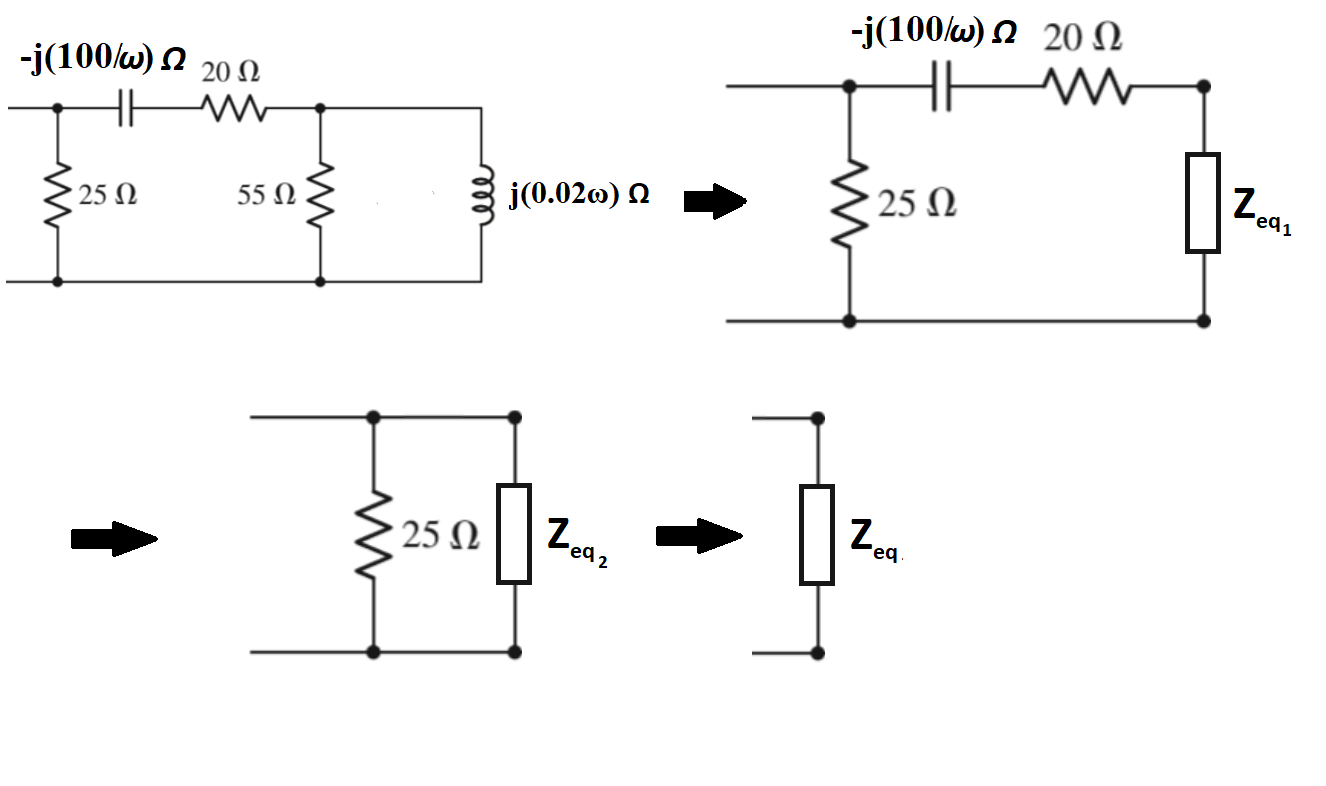
\includegraphics[scale=0.4]{3-06(a).PNG}
	\caption{Equivalencias realizadas no Circuito 3.6}
\end{figure}

Em seguida encontramos a impedância equivalente em série entre o capacitor, o resistor e a impedância $Z_{eq_1}$:

$$Z_{eq_2} = -j100 + 20 + 7\times10^{-6} + j20\times10^{-3}\;\Omega$$
$$Z_{eq_2} = 20,000007 - j99,98 \Omega \Longrightarrow Z_{eq_2} = 101,961\phase{-78,687^\circ}\Omega$$

Assim a resistência vista pelos terminais abertos para $\omega = 1\;rad/s$ é:

$$Z_{eq} = \dfrac{25\phase{0^\circ} \cdot 101,961\phase{-78,687^\circ}}{25\phase{0^\circ} + 101,961\phase{-78,687^\circ}} =\dfrac{2549,03\phase{-78,687^\circ}}{109,64\phase{-65,768^\circ}}$$
$$Z_{eq} = \dfrac{2549,03}{109,64}\phase{-78,687^\circ-(-65,768^\circ)} = 23,2491\phase{-12,919^\circ} \Omega$$
\begin{equation}
    \centering
    \fbox{$Z_{eq} = 22,6517 - j5,1958\;\Omega$}
\end{equation}
\newpage


%--3.6 - Letra B --------------------------------------------------------------------------
Da mesma forma resolvemos para as outras frequências pedidas:

$b)$ Para $\omega = 10\;rad/s$:

Neste caso, $Z_L=j10\cdot20\cdot10^{-3} = j0,2\;\Omega$ e $Z_C=-j\frac{100}{10}=-j10\;\Omega$. Assim:

\begin{equation}
    \centering
    \fbox{$Z_{eq} = 11,74 - j2,88\;\Omega$}
\end{equation}

$c)$ Para $\omega = 100\;rad/s$:

Neste caso, $Z_L=j100\cdot20\cdot10^{-3} = j2\;\Omega$ e $Z_C=-j\frac{100}{100}=-j\;\Omega$. Assim:

\begin{equation}
    \centering
    \fbox{$Z_{eq} = 11,13 + j0,307\;\Omega$}
\end{equation}

\begin{flushright}
    $\Box$
\end{flushright}

\newpage

% ----------------------------------------------------------
% QUESTÃO 3.8
% ----------------------------------------------------------
\section*{Questão 3.8}
\addcontentsline{toc}{section}{Questão 3.8}

Determine $i(t)$:

\begin{figure}[htb]
	\centering
	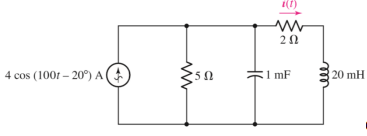
\includegraphics[scale=1]{8.PNG}
	\caption{Circuito 3.8}
\end{figure}

Para a análise no regime permanentemente senoidal, resistores, indutores e capacitores são vistos como impedâncias no circuito. Calculando as impedâncias, tem-se, para o capacitor:

$$Z_C = -j\dfrac{1}{\omega C}$$
$$Z_C = -j\dfrac{1}{100\cdot1\cdot10^{-3}} = -j10 \Omega$$

Para o indutor:

$$Z_L = j\omega L$$
$$Z_L = j\cdot100\cdot20\cdot10^{-3} = j2 \Omega$$
\begin{figure}[htb]
	\centering
	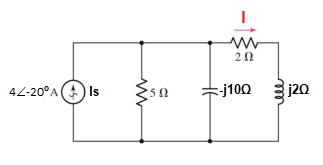
\includegraphics[scale=1]{8-2.PNG}
	\caption{Circuito no domínio da frequência}
\end{figure}

\newpage
Logo, calculando a indutância equivalente entre o resistor de $5\Omega$ e o capacitor de $1\mu F$ em paralelo, tem-se:

$$Z_{eq1} = \dfrac{Z_R\cdot Z_C}{Z_R + Z_C}$$
$$Z_{eq1} = \dfrac{5\cdot (-j10)}{5 - j10}$$
Fazendo transformação para polar:
$$Z_{eq1} = \dfrac{5\phase{0^{\circ}} \cdot 10\phase{-90^{\circ}}}{11,1803\phase{-63,4349^{\circ}}}$$
$$Z_{eq1} = 4,472\phase{-26,565^{\circ}}\;\Omega$$

Para saber a impedância equivalente entre o resistor de $2\Omega$ e o indutor de $20mH$, basta somar os valores:

$$Z_{eq2} = Z_R + Z_L$$
$$Z_{eq2} = 2 + j2 \Omega$$

Como o circuito já está no domínio da frequencia, a fonte de corrente $\textbf{Is}$ tem valor $4\phase{-20^{\circ}} A$, em paralelo com as impedâncias encontradas, $Z_{eq1}$ e $Z_{eq2}$. Logo, para saber a corrente $\textbf{I}$, aplica-se divisor de corrente:

$$\textbf{I} = \dfrac{Z_{eq}}{Z_{eq} + Z_{eq2}}\cdot \textbf{Is}$$
$$\textbf{I} = \dfrac{4,472\phase{-26,565^{\circ}}}{4,472\phase{-26,565^{\circ}} + 2 + j2}\cdot4\phase{-20^{\circ}}$$
$$\textbf{I} = \dfrac{4,472\phase{-26,565^{\circ}}}{4 - j2 + 2 + j2}\cdot4\phase{-20^{\circ}}$$
$$\textbf{I} = \dfrac{17,888\phase{-46,565^{\circ}}}{6\phase{0^{\circ}}}$$
$$\textbf{I} = 2,981\phase{-46,565^{\circ}}\;A$$

Fazendo transformada inversa fasorial para obter $i(t):$

E a corrente máxima é:
\begin{equation}
    \fbox{$i(t) = 2,981\cdot cos(100t - 46,565^{\circ})\;A$}
\end{equation}

\begin{flushright}
    $\Box$
\end{flushright}
\newpage

% ----------------------------------------------------------
% QUESTÃO 3.10
% ----------------------------------------------------------
\section*{Questão 3.10}
\addcontentsline{toc}{section}{Questão 3.10}
Para o circuito 3.10, empregue as técnicas de análise com base em fasores para determinar as duas tensões nodais.
\newline
\begin{figure}[htb]
	\centering
	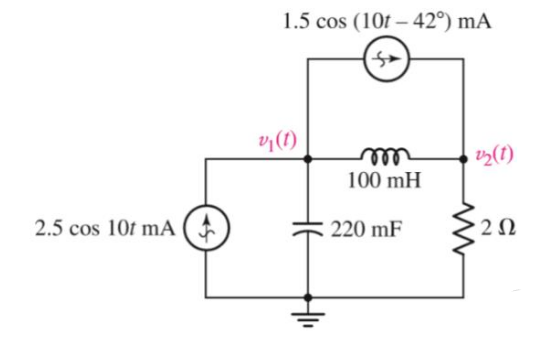
\includegraphics[scale=2]{circuito310.png}
	\caption{Circuito 3.10}
\end{figure}
\newline
Inicialmente encontraremos os valores das impedâncias capacitivas e indutivas. 
$$Z_C = -j\dfrac{1}{w \cdot C} \Longrightarrow Z_C = -j0,4545 \Omega$$
$$Z_L = j(w \cdot L) \Longrightarrow Z_L = j \Omega$$
\begin{figure}[htb]
	\centering
	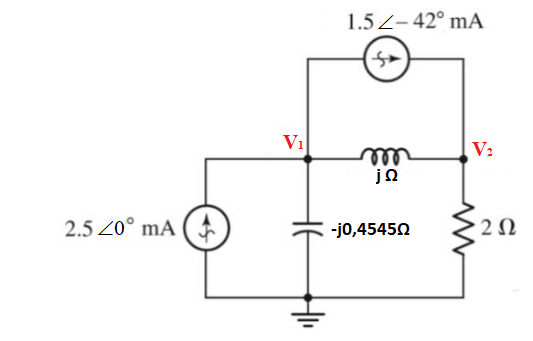
\includegraphics[scale=2]{circuito310-2.png}
	\caption{Circuito no domínio da frequência}
\end{figure}
\newline
Aplicando \textcolor{red}{Análise Nodal} nos pontos indicados $\hat{V_1}$ e $\hat{V_2}$, encontramos:\\
$ Nó_1 $
$$-2,5 \cdot 10^{-3} \measuredangle 0\textsuperscript{o} + \dfrac{\hat{V_1}}{0,4545 \measuredangle -90\textsuperscript{o}} + \dfrac{\hat{V_1} - \hat{V_2}}{1 \measuredangle  90\textsuperscript{o}} + 1,5 \cdot 10^{-3} \measuredangle -42\textsuperscript{o} = 0 $$
$$ \cdot \cdot \cdot $$
\begin{equation}
    \fbox{$1,2j\hat{V_1} + j\hat{V_2} = 1,389 \cdot 10^{-3} + j1,004 \cdot 10^{-3} $}
    \end{equation}\\
$ Nó_2 $
$$ \dfrac{\hat{V_2}}{2} + \dfrac{( \hat{V_2} - \hat{V_1} )}{1 \measuredangle 90\textsuperscript{o}} - 1,5\cdot 10^{-3} \measuredangle -42\textsuperscript{o} = 0$$
$$ \cdot \cdot \cdot $$

\begin{equation}
    \fbox{$j\hat{V_1} + (0,5 - j) \hat{V_2} = 1,115 \cdot 10^{-3} -  j1,004\cdot 10^{-3}$}
\end{equation}

Assim temos o seguinte sistema linear que pode ser escrito da seguinte forma : 
\begin{equation}
    \centering
    \begin{bmatrix}
        1,2j & j \\
        j & (0,5 - j)\\
    \end{bmatrix}
    \cdot
    \begin{bmatrix}
        &\hat{V_1}&\\
        &\hat{V_2}&\\
    \end{bmatrix}
    =
    \begin{bmatrix}
        &1,389 \cdot 10^{-3} + j1,004 &\\
        &1,115 \cdot 10^{-3} -  j1,004\cdot 10^{-3}&\\
    \end{bmatrix}
\end{equation}
O qual aplicando o \textcolor{red}{método de Cramer} para resolução de sistemas lineares temos:
\begin{equation*}
    \centering
    \hat{\Delta} =
    \begin{bmatrix}
        1,2j & j \\
        j & (0,5 - j)\\
    \end{bmatrix}  
\end{equation*}

\begin{equation*}
    \centering
    \hat{N_1}=
    \begin{bmatrix}
         1,389 \cdot 10^{-3} + j1,004 & j \\
         1,115 \cdot 10^{-3} -  j1,004\cdot 10^{-3} & (0,5 - j)\\
    \end{bmatrix}
\end{equation*}

\begin{equation*}
    \centering
        \hat{N_2}=
    \begin{bmatrix}
        1,2j & 1,389 \cdot 10^{-3} + j1,004 \\
        j & 1,115 \cdot 10^{-3} -  j1,004\cdot 10^{-3}\\
    \end{bmatrix}
\end{equation*}\\
O qual podemos encontrar $ \hat{V_1} $ e  $ \hat{V_2} $ aplicando :
\begin{equation*}
    \centering
    \hat{V_i} = \dfrac{det( \hat{N_i} )}{det( \hat{\Delta} )}
\end{equation*}\\
Encontrando os determinantes das Matrizes conhecidas, temos:
    $$det( \hat{\Delta} ) = 2,2 + j0,6 = 2,28\;\phase{15,25^{\circ}} $$
    $$det( \hat{N_1} ) = 0,693 \cdot 10^{-3} - j1,998 \cdot 10^{-3}= 2,115\cdot10^{-3}\;\phase{-70,87^{\circ}}$$ 
    $$det( \hat{N_2} ) = 2,209 \cdot 10^{-3} - j47 \cdot 10^{-6} 
    = 2,209\cdot10^{-3}\;\phase{-1,22^{\circ}}$$\\
Portanto, ao substituir os valores das determinantes, temos que :
\begin{equation}
    \centering
    \hat{V_1} = 928 \cdot 10^{-6} \measuredangle -86,14 \textsuperscript{o} V \Longrightarrow \fbox{ ${v_1} ( t ) = 928 cos (10t-86,14 \textsuperscript{o} ) \mu V $}
\end{equation}
\begin{equation}
    \centering
    \hat{V_2} = 969 \cdot 10^{-6} \measuredangle -16,47 \textsuperscript{o} V \Longrightarrow \fbox{${v_2} ( t )= 969 cos (10t-16,47 \textsuperscript{o} ) \mu V $}
\end{equation}

\begin{flushright}
    $\Box$
\end{flushright}

\newpage

% ----------------------------------------------------------
% QUESTÃO 3.16
% ----------------------------------------------------------

\section*{Questão 3.16} 
\addcontentsline{toc}{section}{Questão 3.16}

Obtenha o equivalente de Thévenin visto pela impedância $(2-j)$ do circuito 3.16 e utilize-o para determinar a corrente $I_1$
%--3.16 -----------------------------

\begin{figure}[htb]
	\centering
	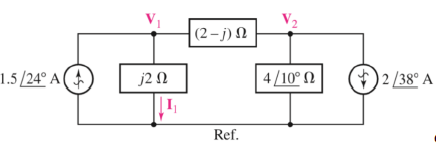
\includegraphics[scale=1]{3-16.PNG}
	\caption{Circuito 3.16}
\end{figure}

Calculando o equivalente de thevenin entre os terminais impedância $(2-j)\;\Omega$
\begin{figure}[htb]
	\centering
	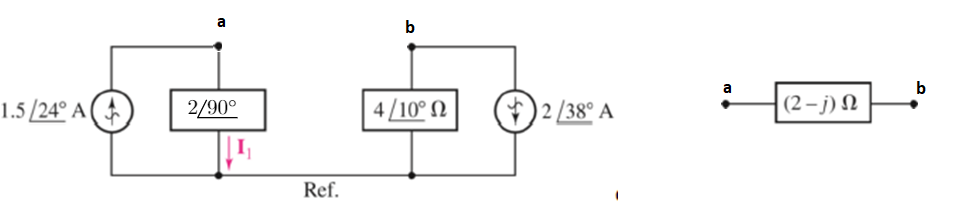
\includegraphics[scale=0.6]{3-16(a).PNG}
	\caption{Circuito 3.16(a)}
\end{figure}

Transformando as fontes:
$$\hat{V_{t_1}} = {1.5 \phase{24^{\circ}}}\cdot{2 \phase{90^{\circ}}}={3 \phase{114^{\circ}}}\;V$$
$$\hat{V_{t_2}} = {-2 \phase{38^{\circ}}}\cdot{4 \phase{10^{\circ}}}={-8 \phase{48^{\circ}}}\;V$$

\begin{figure}[htb]
	\centering
	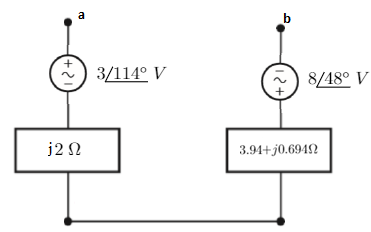
\includegraphics[scale=0.6]{3-16(b).PNG}
	\caption{Circuito 3.16(b)}
\end{figure}

$$\hat{V_{Th}} = {3 \phase{114^{\circ}}}+{8 \phase{48^{\circ}}}={(-1.22+j2.74)+(5.35+j5.9)}\;V$$
$$\hat{V_{Th}} ={4.13+j8.68}={9.61 \phase{64.55^{\circ}}}\;V$$
$$Z_{Th} ={3.94+j0.694+j2}={3.94+j2.694}\;\Omega$$
\newpage
\begin{figure}[htb]
	\centering
	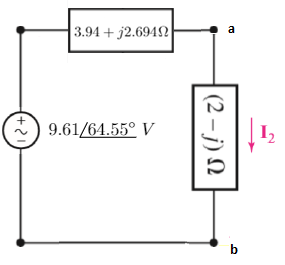
\includegraphics[scale=0.6]{3-16(c).PNG}
	\caption{Circuito 3.16(c)}
\end{figure}

$$\hat{I_2}={\dfrac{\hat{V_{th}}}{Z_{Th}+Z_{(2-j)\;\Omega}}}$$
$$\hat{I_2}={\dfrac{9.61 \phase{64.55^{\circ}}}{3.94+j2.694+2-j}}={\dfrac{9.61 \phase{64.55^{\circ}}}{5.94+j1.694}}={\dfrac{9.61 \phase{64.55^{\circ}}}{6.176 \phase{15.92^{\circ}}}}={1.556 \phase{48.63^{\circ}}}\;A$$
$$\hat{I_2}={1.556 \phase{48.63^{\circ}}}\;A$$
\begin{equation}
    \fbox{$\hat{I_2}={1.556 \phase{48.63^{\circ}}}\;A$}
\end{equation}
No circuito original, temos por LCK:
$$\hat{I_{f1.5\;A}}+\hat{I_1}+\hat{I_2}=0$$
$$\hat{I_1}=\hat{I_{f1.5\;A}}-\hat{I_2}$$
$$\hat{I_1}={1.5 \phase{24^{\circ}}}-{1.556 \phase{48.63^{\circ}}}$$
$$\hat{I_1}=1.37+j0.6401-(1.028+j1.1677)$$
$$\hat{I_1}=0.342-j0.5576$$
$$\hat{I_1}={654.127 \phase{-58.47^{\circ}}}\;mA$$
\begin{equation}
    \fbox{$\hat{I_1}={654.127 \phase{-58.47^{\circ}}}\;mA$}
\end{equation}

\begin{flushright}
    $\Box$
\end{flushright}

\newpage

% ----------------------------------------------------------
% QUESTÃO 3.21
% ----------------------------------------------------------
\section*{Questão 3.21} 
\addcontentsline{toc}{section}{Questão 3.21}

Para o circuito RLC série do circuito 3.21 calcule a tensão em cada elemento e compare-a à corrente do circuito
%--3.21 -----------------------------
\begin{figure}[htb]
	\centering
	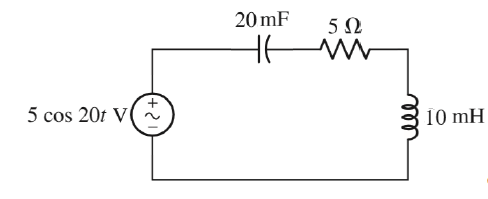
\includegraphics[scale=1]{3-21.PNG}
	\caption{Circuito 3.21}
\end{figure}

\begin{figure}[htb]
	\centering
	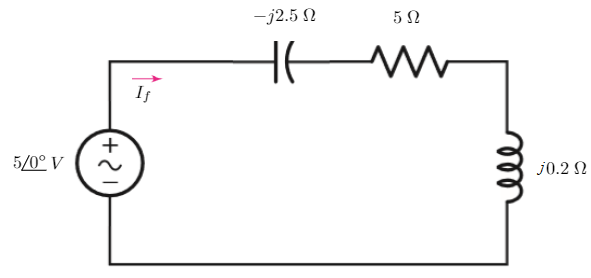
\includegraphics[scale=0.7]{3-21(a).PNG}
	\caption{Circuito 3.21(a)}
\end{figure}


$$Z_c = -j{\dfrac{1}{\omega\cdot C}}=-j{\dfrac{1}{20\cdot 20\times 10^{-3}}}=-j2.5\;\Omega$$
$$Z_L=j\omega \cdot L=j20\cdot20\times10^{-3}=j0.2\;\Omega$$
$$\hat{I_f}={\dfrac{\hat{V_f}}{Z_{ec}}}$$
$$\hat{I_f}={\dfrac{{5 \phase{0^{\circ}}}}{-12.5+5+j0.2}}={\dfrac{{5 \phase{0^{\circ}}}}{5-j2.3}}={\dfrac{{5 \phase{0^{\circ}}}}{{5.503 \phase{-24.70^{\circ}}}}}$$
\begin{equation}
   \fbox{$\hat{I_f}={908.595 \phase{24.70^{\circ}}}\;mA$}
\end{equation}
$$\hat{V_c}=Z_c\cdot \hat{I_f}$$
$$\hat{V_c}={2.5 \phase{-90^{\circ}}}\cdot{908.595\times10^{-3} \phase{-24.70^{\circ}}}={2.27 \phase{-65.3^{\circ}}}\;V$$
\begin{equation}
    \fbox{$\hat{V_c}={2.27 \phase{-65.3^{\circ}}}\;V$}
\end{equation}
A corrente no capacitor está adiantada $90^{\circ}$ em relação a tensão.
$$\hat{V_L}=Z_L\cdot \hat{I_f}$$
$$\hat{V_L}={0.2 \phase{90^{\circ}}}\cdot{908.595\times10^{-3} \phase{24.70^{\circ}}}={181.719 \phase{114.70^{\circ}}}\;mV$$
\begin{equation}
    \fbox{$\hat{V_L}={181.719 \phase{114.70^{\circ}}}\;mV$}
\end{equation}
A corrente no indutor está atrasada $90^{\circ}$ em relação a tensão.
$$\hat{V_R}=R\cdot \hat{I_f}$$
$$\hat{V_R}=5\cdot{908.595\times10^{-3} \phase{24.70^{\circ}}}={4.54 \phase{24.70^{\circ}}}\;V$$
\begin{equation}
    \fbox{$\hat{V_R}={4.54 \phase{24.70^{\circ}}}\;V$}
\end{equation}
A corrente está em fase com a tensão nos terminais do resistor.

\begin{flushright}
    $\Box$
\end{flushright}

\newpage

% ----------------------------------------------------------
% QUESTÃO 3.23
% ----------------------------------------------------------

\section*{Questão 3.23}
\addcontentsline{toc}{section}{Questão 3.23}

Com base no Circuito 3.23, dê o valor (em Henrys ou Farads) do elemento que deve ser colocado em série com a fonte de tensão para que a corrente fornecida não esteja defasada da tensão aplicada.

\begin{figure}[htb]
	\centering
	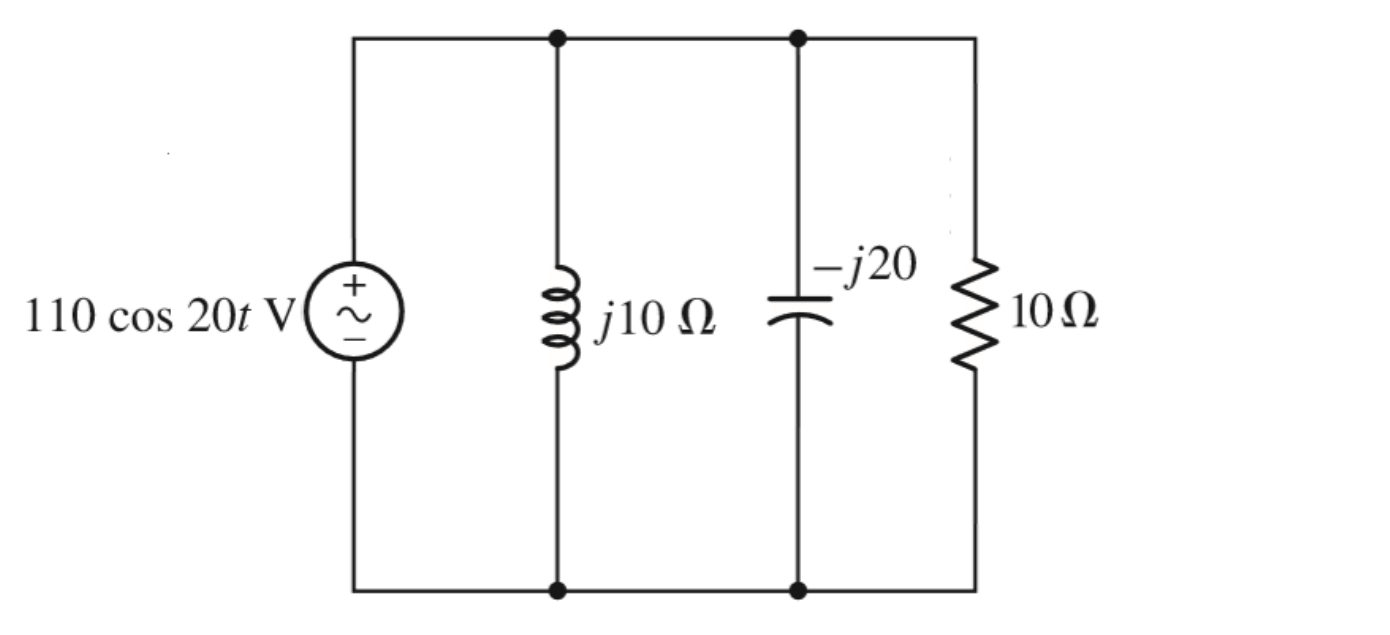
\includegraphics[scale=1]{circuito323.png}
	\caption{Circuito 3.23}
\end{figure}

Primeiramente deveremos encontrar a \textcolor{red}{Impedância equivalente} $Z_{eq}$

\begin{equation*}
    \centering
    \dfrac{1}{Z_{eq}} = \dfrac{1}{10 \measuredangle 90 \textsuperscript{o} } + \dfrac{1}{20 \measuredangle -90\textsuperscript{o}} + \dfrac{1}{10} 
\end{equation*}

\begin{equation*}
    \centering
    \dfrac{1}{Z_{eq}} = 0,1 \measuredangle -90 \textsuperscript{o}  + 0,05 \measuredangle 90\textsuperscript{o} + 0,1 \Longrightarrow \dfrac{1}{Z_{eq}} = -j0,1 + j0,05 + 0,1
\end{equation*}

\begin{equation}
    \centering
    Z_{eq} = 8 + j4 \Omega;
\end{equation}

Sabemos que a para eliminar a componente imaginária de $Z_{eq}$, devemos inserir uma reatância de mesmo módulo, com sentido oposto e em série com fonte do circuito, portanto $ X = -4 $.
Como $X < 0$ então \textcolor{red}{a reatância é capacitiva}, assim temos : 
$$ X = \dfrac{-1}{w\cdot C}$$
$$ -4 = \dfrac{-1}{20 \cdot C} \longrightarrow C = \dfrac{1}{80}$$

\begin{equation}
    \centering
    \fbox{$C = 12,5 mF$}
\end{equation}

Assim, deve-se adicionar um capacitor de $12,5 mF$ em série com a fonte de tensão, para que corrente e tensão na fonte tenham a mesma fase.

\begin{flushright}
    $\Box$
\end{flushright}
\newpage

% ----------------------------------------------------------
% QUESTÃO 3.25
% ----------------------------------------------------------

\section*{Questão 3.25}
\addcontentsline{toc}{section}{Questão 3.25}

Determine a corrente $\textbf{I}$:

\begin{figure}[htb]
	\centering
	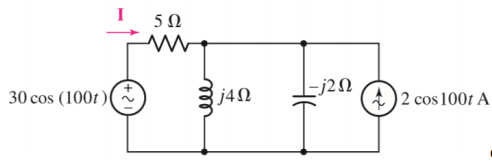
\includegraphics[scale=0.8]{25.PNG}
	\caption{Circuito 3.25}
\end{figure}

Calculando a contribuição da fonte de tensão para a corrente $\textbf{I}$:

\begin{figure}[htb]
	\centering
	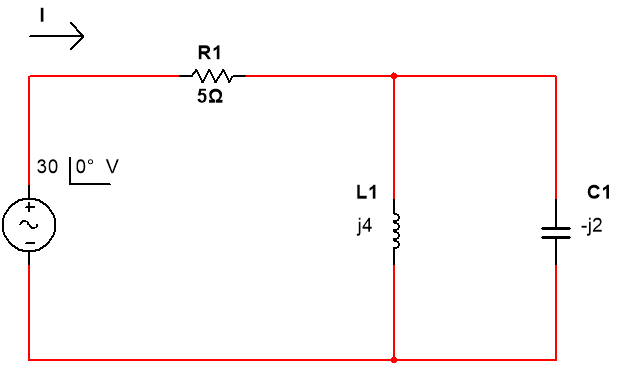
\includegraphics[scale=0.4]{25_1.PNG}
\end{figure}

$$Z_{eq1} = \dfrac{Z_L\cdot Z_C}{Z_L + Z_C}$$
$$Z_{eq1} = \dfrac{4\phase{90^{\circ}}\cdot 2\phase{-90^{\circ}}}{j4 - j2}$$
$$Z_{eq1} = \dfrac{8\phase{0^{\circ}}}{2\phase{90^{\circ}}}$$
$$Z_{eq1} = 4\phase{-90^{\circ}}\;\Omega$$
$$Z_{eq1} = -j4\;\Omega$$

Calculando a impedância equivalente em série:

$$Z_{eq} = Z_R + Z_{eq1}$$
$$Z_{eq} = 5 - j4\;\Omega$$

A contribuição pela fonte de tensão de $30\phase{0^{\circ}}\;V$ será:

$$\textbf{I'} = \dfrac{\textbf{V'}}{Z_{eq}}$$
$$\textbf{I'} = \dfrac{30\phase{0^{\circ}}}{5 - j4}$$
$$\textbf{I'} = \dfrac{30\phase{0^{\circ}}}{6,403\phase{-38,657^{\circ}}}$$
$$\textbf{I'} = 4,6853\phase{38,659^{\circ}}\;A$$
$$\textbf{I'} = 3,6586 + j2,9268\;A$$

Calculando a contribuição da fonte de corrente de $2\phase{0^{\circ}}\;A$:

\begin{figure}[htb]
	\centering
	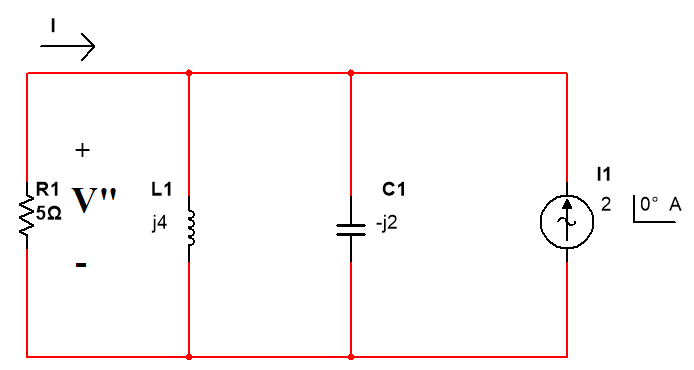
\includegraphics[scale=0.4]{25_2.PNG}
\end{figure}

A impedância equivalente em paralelo será dada por:

$$\dfrac{1}{Z_{eq2}} = \dfrac{1}{Z_R} + \dfrac{1}{Z_L} + \dfrac{1}{Z_C}$$
$$\dfrac{1}{Z_{eq2}} = 0,2 - j0,25 + j0,5$$
$$Z_{eq2} = 3,123\phase{-51,34^{\circ}}\;\Omega$$
Calculando a tensão no paralelo,temos:
$$\textbf{V''} = Z_{eq2}\cdot \textbf{I$_f$} $$
$$\textbf{V''} = 3,123\phase{-51,34^{\circ}}\cdot 2\phase{0^{\circ}}$$
$$\textbf{V''} = 6,246\phase{-51,34^{\circ}}\;V$$


Pela lei de ohm, temos que a corrente no resistor de 5$\Omega$ é:
\newline
$$\textbf{V''} = -Z_{R}\cdot \textbf{I''} $$
$$\textbf{I''} = -\dfrac{\textbf{V''}}{Z_R}$$
$$\textbf{I''} = \dfrac{-6,246\phase{-51,34^{\circ}}}{5}\;A$$
$$\textbf{I''} = -1,249\phase{-51,34^{\circ}}\;A$$
$$\textbf{I''} = -780,247\cdot10^{-3} + j975,303\cdot10^{-3}\;A$$

\newpage

Por LCK:
$$\textbf{I} = \textbf{I'} + \textbf{I''}$$

Logo:
$$\textbf{I} = 3,6586 + j2,9268 -780,247\cdot10^{-3} + j975,303\cdot10^{-3}$$
$$\textbf{I} = 2,8784 + j3,9021\;A$$
$$\textbf{I} = 4,8489\phase{\;53,58^{\circ}}\;A$$

\begin{flushright}
    $\Box$
\end{flushright}
\newpage

% ----------------------------------------------------------
% QUESTÃO 3.35
% ----------------------------------------------------------

\section*{Questão 3.35}
\addcontentsline{toc}{section}{Questão 3.35}
Para o Circuito 3.35, obtenha os equivalentes de Thévenin e Norton nos terminais $a-b$.
\begin{figure}[htb]
	\centering
	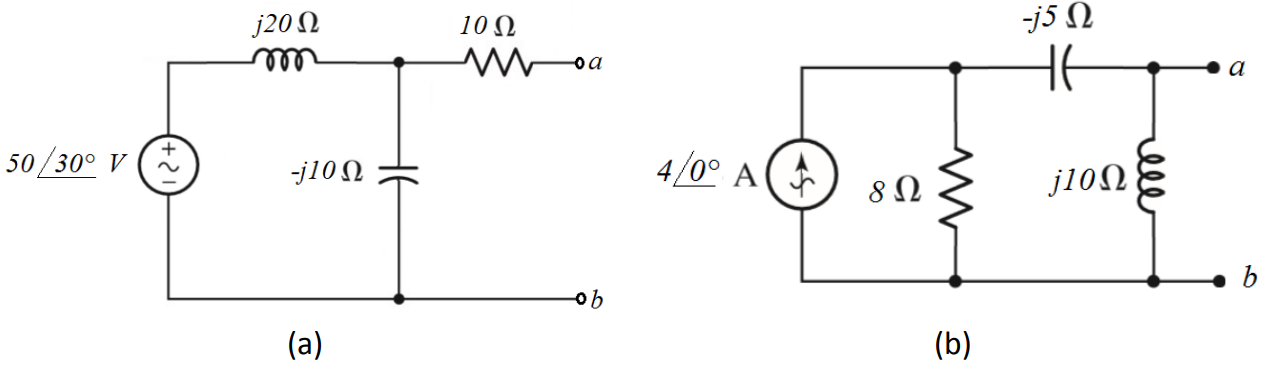
\includegraphics[scale=0.5]{3-35.PNG}
	\caption{Circuitos 3.35 (a) e (b)}
\end{figure}

%--3.35 - Letra A -------------------------------------------------------------------------
$a)$ Para o Circuito 3.35(a):

Pelo método das tensões de nó:
$$\dfrac{\hat{V_{TH}}}{10\phase{-90^{\circ}}}+\dfrac{(\hat{V_{TH}}-50\phase{30^{\circ}})}{20\phase{90^{\circ}}}=0$$
$$j0,1\cdot \hat{V_{TH}} + (\hat{V_{TH}} - 50\phase{30^{\circ}}) \cdot 0,05\phase{-90^{\circ}} = 0$$
$$j0,1\cdot \hat{V_{TH}} + (-j0,05\hat{V_{TH}} - 2,5\phase{-90^{\circ}}) = 0$$
$$\hat{V_{TH}}\cdot 0,05\phase{90^{\circ}}=2,5\phase{60^{\circ}}$$
$$\hat{V_{TH}}=\dfrac{2,5\phase{-60^{\circ}}}{0,05\phase{90^{\circ}}} = 50\phase{-150^{\circ}}\;V$$

Calculando $Z_{TH}$:
\begin{paracol}{2}
\begin{figure}[htb]
	\centering
	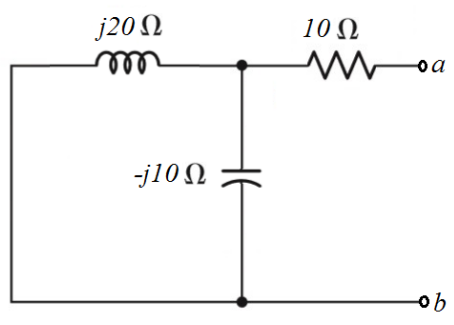
\includegraphics[scale=0.5]{3-35(a).PNG}
	\caption{Impedância equivalente}
\end{figure}
\switchcolumn
$$Z_{ab} = \frac{20\phase{90^{\circ}}\cdot 10\phase{-90^{\circ}}}{j20-j10}+10\;\Omega$$
$$Z_{ab} = \frac{20\phase{0^{\circ}}}{10\phase{90^{\circ}}}+10=20\phase{-90^{\circ}}\;+10\Omega$$
$$Z_{ab} = 10-j20 \Omega = 22,36\phase{-63,43^{\circ}}\;\Omega$$
\end{paracol}
\newpage

Tendo obtida a impedância vistas pelos terminais a-b $Z_{ab}$ e a tensão de Thévenin $\hat{V_{TH}}$, obtemos a corrente de Nórton $\hat{I_N}:$

$$\hat{I_N} = \dfrac{\hat{V_{TH}}}{Z_{ab}}=\dfrac{50\phase{-150^{\circ}}\;V}{22,36\phase{-63,43^{\circ}}\;\Omega} = 2,236\phase{-86,57^{\circ}}\;\Omega$$

Assim obtemos os circuitos equivalente para o Circuito 3.35(a) :

\begin{figure}[htb]
	\centering
	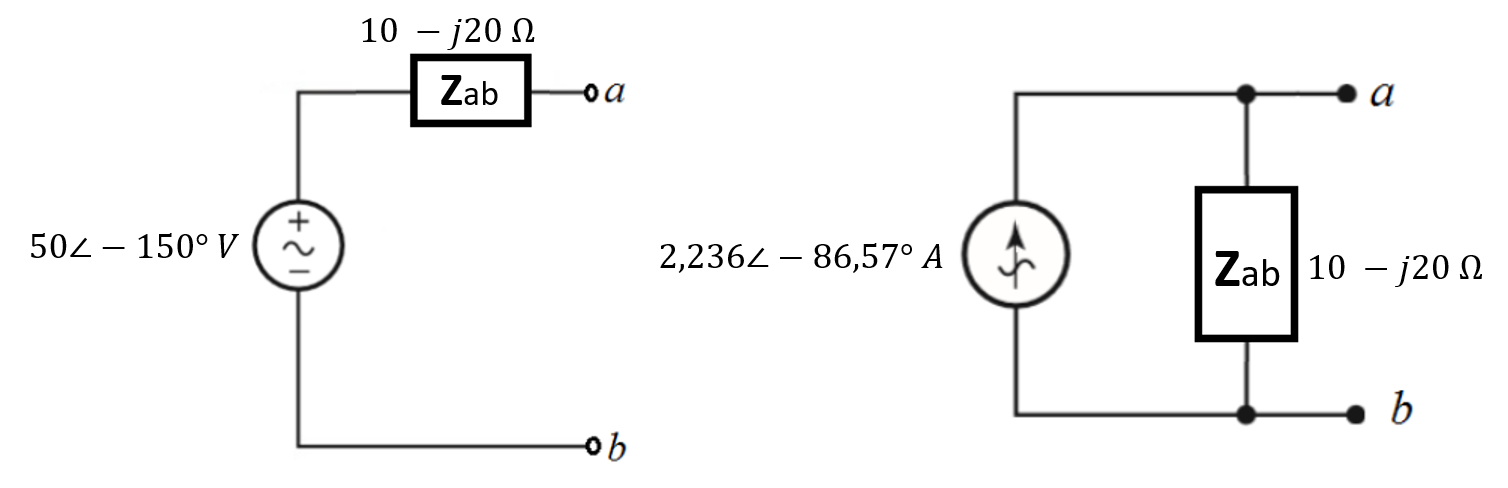
\includegraphics[scale=0.35]{3-35(b).PNG}
	\caption{Circuitos Equivalentes Thévenin e Nórton}
\end{figure}

$b)$ Para o Circuito 3.35(b), inicialmente utilizamos transformação de fonte de corrente para de tensão:
$$\hat{V_{TH}} = 4\phase{0^{\circ}}\cdot 8 = 32\phase{0^{\circ}} V$$

\begin{figure}[htb]
	\centering
	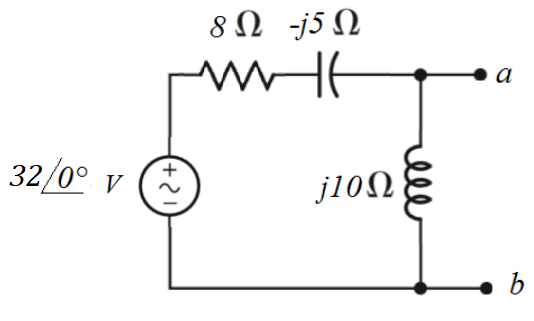
\includegraphics[scale=0.5]{3-35(c).PNG}
\end{figure}

Utilizando transformação de fonte de tensão para de corrente, temos:
$$\hat{I_N} = \dfrac{32\phase{0^{\circ}}}{9,433\phase{-32^{\circ}}} = 3,39\phase{32^{\circ}} A$$

\begin{figure}[htb]
	\centering
	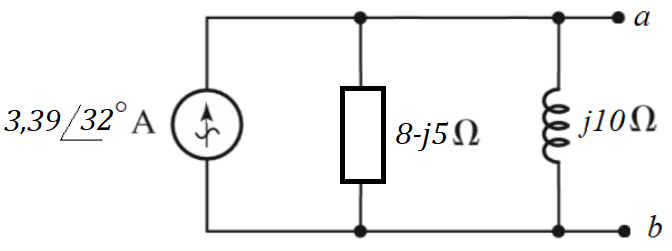
\includegraphics[scale=0.5]{3-35(d).PNG}
\end{figure}

\newpage
Calculando $Z_N$ que é obtida através da associação em paralelo das impedâncias vista no circuito anterior, temos:
$$Z_N = \dfrac{9,433\phase{-32^{\circ}} \cdot 10\phase{90^{\circ}}}{8-j5+j10}$$
$$Z_N = \dfrac{94,33\phase{58^{\circ}}}{9,43\phase{32^{\circ}}} = 10\phase{26^{\circ}}$$
$$Z_N = 8,987 + j4,383 \Omega$$

Assim obtemos o equivalente de Norton:

\begin{figure}[htb]
	\centering
	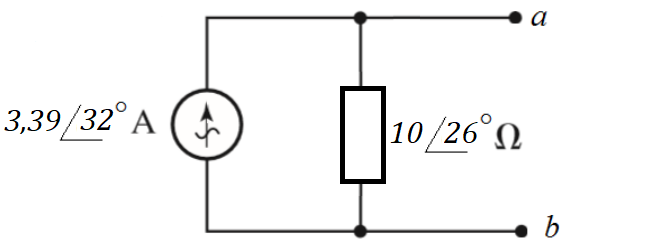
\includegraphics[scale=0.5]{3-35(e).PNG}
\end{figure}

Por fim obtemos o equivalente de Thévenin da seguinte maneira:
$$\hat{V_{TH}} = 3,39\phase{32^{\circ}} \cdot 10\phase{26^{\circ}} = 33,9\phase{58^{\circ}} V$$

\begin{figure}[htb]
	\centering
	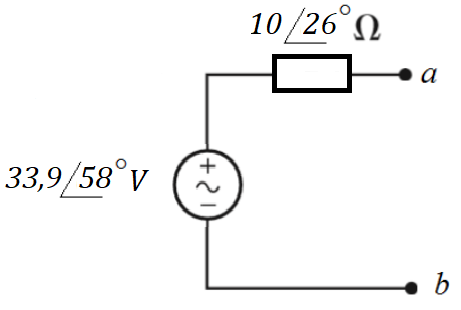
\includegraphics[scale=0.5]{3-35(f).PNG}
\end{figure}

\begin{flushright}
    $\Box$
\end{flushright}
\newpage

% ----------------------------------------------------------
% QUESTÃO 3.39
% ----------------------------------------------------------
\section*{Questão 3.39}
\addcontentsline{toc}{section}{Questão 3.39}
Um circuito RL série operando em regime permanente é alimentado por uma fonte de tensão CA. Se a frequência da fonte aumentar, mas sua amplitude permanecer constante, pode-se afirmar que:


$(a)$ a amplitude da corrente não se altera; 

$(b)$ a amplitude da corrente aumenta;

$(c)$ a frequência da corrente diminui;

$(d)$ o ângulo de atraso da corrente em relação à tensão aumenta.

\begin{figure}[htb]
	\centering
	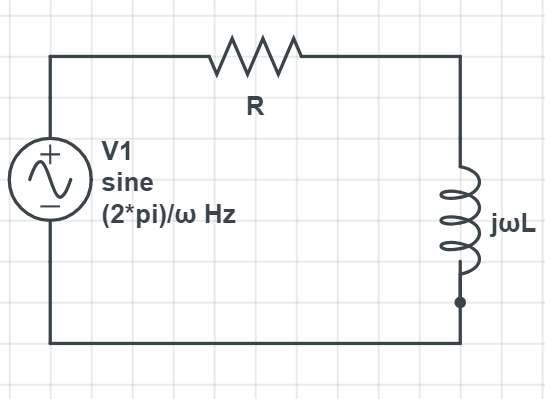
\includegraphics[scale=0.65]{circuito_3-39.png}
	\caption{Circuito RL}
\end{figure}

$a)$ Falso, pois {$Z_L$} depende de $\omega$, logo se ocorrer um aumento de freqência, ocorre variação da impedância equivalente do circuito e isso causa uma variação na amplitude de corrente.

$b)$ Falso, ela diminui pois houve um aumento da frequência, portanto a impedância equivalente do circuito aumentou.

$c)$ Falso, pois se a frequência na fonte aumentou, a frequência em todo o circuito aumentou igualmente, logo a frequência da corrente aumenta.

$d)$ Verdadeiro, pois como a parte imaginária da impedância equivalente aumenta, há um aumento da influência da parcela indutiva no circuito, aumentando o atraso da corrente em relação a tensão.

\begin{flushright}
    $\Box$
\end{flushright}
\newpage
%==========================================================================================


% ----------------------------------------------------------
% Finaliza a parte no bookmark do PDF
% para que se inicie o bookmark na raiz
% e adiciona espaço de parte no Sumário
% ----------------------------------------------------------
\phantompart

% ----------------------------------------------------------
% ELEMENTOS PÓS-TEXTUAIS
% ----------------------------------------------------------
\postextual
% ----------------------------------------------------------

% ----------------------------------------------------------
% Referências bibliográficas
% ----------------------------------------------------------
\bibliography{abntex2-modelo-references}

\end{document}
